\documentclass{article}

\usepackage{fancyhdr}
\usepackage{mathtools}
\usepackage{amsmath}

\pagestyle{fancy}

\lhead{Robin Touche 900610-3270}
\rhead{robint@student.chalmers.se}

\begin{document}
\chapter{Homework 1}
\setcounter{section}{1}
\subsection{}

To find $\sigma$ we need to try to maximise the likelihood function
$\mathcal{L}$ given as the probability density function $f(x_1, x_2, ... , x_n
\vert \theta)$ where $\theta = (\mu, \sigma^2)$.

The probability density function is given by:

\begin{align}
  f(\mathbf{x} \vert \mu , \sigma^2) = \frac{1}{2\pi^{p / 2} \sigma}
  \cdot e^{\left( - \frac{1}{2} \left( \mathbf{x} - \mu \right) ^T
  \sigma^2 \left(\mathbf{x} - \mu \right) \right)}
\end{align}

The likelihood function can be simplified to:

\begin{align}
  \mathcal{L}(\theta ; \mathbf{x}) &= \prod_{i = 1}^{n}f(x_i \vert \theta) =\\
  \notag &= \left( \frac{1}{\sigma\sqrt{2\pi}^{p}} \right) ^n
    \cdot e^{\left( - \frac{1}{2} \sum_{i = 1}^{n}
    \notag \left( x_i - \mu \right) ^T \sigma^2 \left(x_i - \mu \right) \right)}
\end{align}

To get rid of the annoying exponent we can instead work with the natural
logarithm of $\mathcal{L}$.

\begin{align}
  ln(\mathcal{L}) = - \frac{n}{2} ln(2\pi) - ln(\sigma)
    - \frac{1}{2} \sum_{i = 1}^{n}
    \left( x_i - \mu \right) ^T \sigma^2 \left(x_i - \mu \right)
\end{align}

Since we want to maximise this we can find $\sigma$ s.t. the derivative
$\frac{d}{d\sigma}ln(\mathcal{L}) = 0$.

\begin{align}
  \frac{d}{d\sigma}ln(\mathcal{L}) = -\frac{n}{\sigma} + \frac{1}{\sigma^3}
  \sum_{i = 1}^{n} \left( x_i - \mu \right) ^T \left(x_i - \mu \right) \Rightarrow \\
  \sigma^2 = \frac{1}{n} \sum_{i = 0}^{n - 1}
    \left( x_i - \hat{x} \right) \left(x_i - \hat{x} \right)^T
\end{align}

where $\hat{x}$ is the expected value of $x$.

\subsection{}
\paragraph{a)}

\begin{align*}
  P(\sigma^2 | \mathbf{x}, \mu) &\propto
  \prod_{i = 1}^{n} \Bigg( \frac{1}{2\pi\sigma^2}
    exp{\left( - \frac{(x_i - \mu)^T(x_i - \mu)}{2\sigma^2} \right)} \Bigg) \cdot
    \left( \frac{\beta_{0}^{\alpha_0}}{\Gamma (\alpha_0)}
    {\sigma^2}^{- \left( \alpha_0 + 1 \right)}
    exp \left( - \frac{\beta_0}{\sigma^2} \right) \right) \\
  &\propto \prod_{i = 1}^{n} \Bigg( \sigma^{-2}
    exp{\left( - \frac{(x_i - \mu)^T(x_i - \mu)}{2\sigma^2} \right)} \Bigg) \cdot
    \left( {\sigma^2}^{- \left( \alpha_0 + 1 \right)}
    exp \left( - \frac{\beta_0}{\sigma^2} \right) \right) \\
  &= \sigma^{-2n} exp \left( - \sum_{i = 1}^{n}
    \frac{(x_i - \mu)^T(x_i - \mu)}{2\sigma^2} \right) \cdot
    {\sigma^2}^{- \left( \alpha_0 + 1 \right)}
    exp \left( - \frac{\beta_0}{\sigma^2} \right) \\
  &= {\sigma^2}^{- \left( n + \alpha_0 + 1 \right)}
    exp \Bigg( - \left( \frac{\beta_0}{\sigma^2} + \frac{\sum_{i = 1}^{n}
    (x_i - \mu)^T(x_i - \mu)}{2\sigma^2} \right) \Bigg) \\
  &= {\sigma^2}^{- \left( n + \alpha_0 + 1 \right)}
    exp \left( - \frac{\beta_0 + \frac{\sum_{i = 1}^{n}
    (x_i - \mu)^T(x_i - \mu)}{2}}{\sigma^2} \right)
\end{align*}

From this we can derive $\alpha_1$ and $\beta_1$ as:

\begin{align*}
  \alpha &= \alpha_0 + n \\
  \beta  &= \beta_0 + \frac{\sum_{i = 1}^{n} (x_i - \mu)^T(x_i - \mu)}{2}
\end{align*}

Which gives us a posterior distribution of

\begin{align*}
  \text{invgamma} \left( \alpha_0 + n, \beta_0 +
  \frac{\sum_{i = 1}^{n} (x_i - \mu)^T(x_i - \mu)}{2} \right)
\end{align*}

\paragraph{b)}

The Bayes factor $K$ is given by

\begin{align*}
  K &= \frac{P \left( D \vert M_a \right)}{P \left( D \vert M_b \right)} \\
  &= \frac{ \int P \left( \theta_a \vert M_A \right) P \left( D \vert \theta_a , M_A \right) d \theta_a}
  { \int P \left( \theta_b \vert M_B \right) P \left( D \vert \theta_b , M_B \right) d \theta_b} \\
  &= \frac{ \displaystyle \int \frac{\beta_{a}^{\alpha_a}}{\Gamma (\alpha_a)}
    {\sigma^2}^{-(\alpha_a + 1)} exp \left( - \frac{\beta_a}{\sigma^2} \right)
    \frac{1}{2\pi\sigma^2}
    exp{\left( - \frac{(x_i - \mu)^T(x_i - \mu)}{2\sigma^2} \right)}}
    { \displaystyle \int \frac{\beta_{b}^{\alpha_b}}{\Gamma (\alpha_b)}
    {\sigma^2}^{-(\alpha_b + 1)} exp \left( - \frac{\beta_b}{\sigma^2} \right)
    \frac{1}{2\pi\sigma^2}
    exp{\left( - \frac{(x_i - \mu)^T(x_i - \mu)}{2\sigma^2} \right)}}
\end{align*}

\paragraph{c)}

First we need to calculate $\hat{\sigma}^2_{MAP}$ as

\begin{align*}
  \hat{\sigma}^2_{MAP}
    &= argmax_{\sigma^2} \text{P} \left( \sigma^2 \right) \text{P} \left( D \vert \sigma^2 \right) \\
    &= argmax_{\sigma^2} log \text{P} \left( D \vert \sigma^2 \right) + log \text{P} \left( \sigma^2 \right)
\end{align*}

We derive this to find a stationary point (\emph{i.e} a maximum in this case).

\begin{align*}
  & \frac{d}{d\sigma^2} \hat{\sigma}^2_{MAP} \\
  &= \frac{d}{d\sigma^2} \Bigg( ln \Bigg( \frac{1}{2\pi\sigma^2}
    exp{\left( - \frac{(x_i - \mu)^T(x_i - \mu)}{2\sigma^2} \right)} \Bigg) +
    ln \Bigg( \frac{\beta_{0}^{\alpha_0}}{\Gamma (\alpha_0)}
    {\sigma^2}^{- \left( \alpha_0 + 1 \right)} \Bigg)
    exp \left( - \frac{\beta_0}{\sigma^2} \right) \Bigg) \\
  &= \frac{d}{d\sigma^2} \Bigg( ln \left( \frac{1}{2\pi\sigma^2} \right)
    {\left( - \frac{(x_i - \mu)^T(x_i - \mu)}{2\sigma^2} \right)} +
    ln \left( \frac{\beta_{0}^{\alpha_0}}{\Gamma (\alpha_0)} \right)
    {\sigma^2}^{- \left( \alpha_0 + 1 \right)}
    \left( - \frac{\beta_0}{\sigma^2} \right) \Bigg)
\end{align*}

\setcounter{section}{2}
\setcounter{subsection}{0}
\subsection{}
\paragraph{a)}

By using the logarithm likelihood function as above we can estimate $\mu$ as:

\begin{align}
  \mu = \frac{1}{n} \sum_{i = 1}^{n} x_n
\end{align}

We can use this $\mu$ to calcualte $\sigma$ as:

\begin{align}
  \sigma = \frac{1}{n} \sum_{i = 1}^{n} (x_n - \mu)(x_n - \mu)^T
\end{align}

\paragraph{b, c)}
See code

\paragraph{d)}
\begin{figure}[H]
\centering
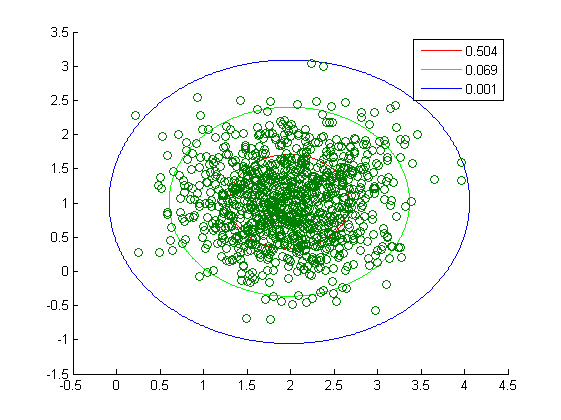
\includegraphics[scale=0.7]{Fig21.png}
\end{figure}

\end{document}
